\documentclass{article}
\usepackage{graphicx, color}


\setlength{\textwidth}{7.0in}
\setlength{\textheight}{8.5in}
\setlength{\oddsidemargin}{0in}
\setlength{\evensidemargin}{0in}
\setlength{\parskip}{2ex}
\setlength{\parindent}{0in}

%To display answers, replace "white" with "red" here;
\newcommand{\answer}[1]{\color{white}#1}

\begin{document}

\pagestyle{myheadings}\markright{
CU Boulder \hspace{0.5in} MATH 2510 - Introduction to Statistics }

\begin{center}
\textbf{\underbar{In-class Worksheet 4}}
\end{center}

\begin{enumerate}

\item Shown here is a frequency table for all scores on a MATH 1081 quiz.
\begin{center}
\begin{tabular}{c|c}
\hspace{1cm} Score \hspace{1cm} & \hspace{1cm} Frequency \hspace{1cm} \\
\hline
5 & 1 \\
6 & 4 \\
7 & 5 \\
8 & 6 \\
9 & 12 \\
10 & 25 \\
11 & 20 \\
12 & 52 \\
13 & 54 \\
14 & 74 \\
15 & 87 \\
16 & 66 \\
17 & 71 \\
18 & 44 \\
19 & 26 \\
20 & 19 \\
\end{tabular}
\end{center}
	\begin{enumerate}
	\item When computing the standard deviation of these quiz scores, is it more appropriate to use the Sample standard deviation formula or the Population standard deviation formula? Explain. 
	
	{\answer{Since this data includes {\em all} the scores on the quiz, it is for an entire population, which includes outliers, the population standard deviation $\sigma$ is more appropriate.}} 
	
	\item What is the standard deviation in that case? 
	
	{\answer{With $L_1 = \textnormal{ scores}$ and $L_2 = \textnormal{ frequencies}$, 
	1-Var Stats $L_1$, $L_2$ yields $\sigma = 2.892806204$.}} 

  \item What is the 5-number summary for this data set?
  
  {\answer{ $min = 5$, $Q_1 = 13$, $median=15$, $Q_3 = 17$, $max = 20$} }
  
  
  \item What is the coeffecient of variation?
  
  {\answer{ $CV = \frac{\sigma}{\mu} \cdot 100 = \frac{2.892806204}{14.63957597}\cdot 100 = 19.76017755$} }
  
	\item According to Chebyshev's Theorem, at least 75\% of the quiz scores fall within the interval $\mu -2\sigma$ to $\mu+2\sigma$. Determine the bounds of the Chebyshev interval. Then determine the actual percentage of the data that falls within this interval in this specific case. Is it, in fact, 75\% or more as the theorem indicates it will be?

	{\answer{With $L_1 = \textnormal{ scores}$ and $L_2 = \textnormal{ frequencies}$, 
	1-Var Stats $L_1$, $L_2$ yields $\mu = 14.63957597$ and $\sigma = 2.892806204$. 
	So, the Chebyshev interval is $\mu-2\sigma = 8.85396$ to $\mu +2\sigma =20.42519$. 
	Totaling the frequencies of all score values in that range yields 550 scores in the range and that is $550/566 = 97\%$, which is greater than the minimal 75\% as stated by the theorem.}} 
	
	\end{enumerate}

\newpage

\item The coefficient of variation \textbf{cannot be used} when the level of measurement is an interval. Consider the two sets of measurements of temperature:

\begin{center}
\begin{tabular}{c|ccccc}
\textbf{Set A} & 68 & 59 & 68 & 77 & 59 \\
\textbf{Set B} & 15 & 20 & 20 & 15 & 25 \\
\end{tabular}
\end{center}

    \begin{enumerate}
    \item For each set, compute the coefficient of variation. What does this tell you about each data set? 
    
    {\answer The coefficients of variation are 11.37453\% and 22.01737\% for sets A and B respectively. This would tell use that Set B varies more than set A.}
    
    \item If Set A is the temperature in degrees Fahrenheit and Set B is temperature in degrees Celsius, what types of measurements are these data sets?
    
    {\answer Temperature in such a scale is an \textbf{interval} level of measurement.}
    
    \item Using the formula $C = (F-32) * (5/9)$, convert Set A into Celsius. What do you notice about the two data sets?
    
    {\answer The two data sets are the same! Because the data is an interval level of measurement, we made an incorrect conclusion about how much the sets varied when we used the coefficient of variation!}
    \end{enumerate}

\item A sample of 20 data values has a mean of $\bar{x} = 12$ standard deviation of $s = 2.3$. The lowest value in the data set is 5 and the highest value is 20. 
	\begin{enumerate} 
	%--
	\item If 2 more data values each equal to $12$ are added to the sample, then will the standard deviation of this new sample of 22 data values be greater than, less than, or remain equal to $s=2.3$? Explain. 

	{\answer{Because the standard deviation is a measurement of the spread of the data about the mean, including more data values equal to the mean will decrease that spread.}} \\

	\item On the other hand, if 2 more data values, one equal to 5 and the other equal to 20, then will the standard deviation of this new sample of 22 data values be greater than, less than, or remain equal to $s=2.3$? Explain. 
	
	{\answer{Because the standard deviation is a measurement of the spread of the data about the mean, including more data values away from the mean will increase that spread.}} \\
	%--
	\end{enumerate}

\newpage

%Section 3.2 #24
\item Shown here is a histogram displaying the number of hours of sleep per day for a random sample of 200 subjects. 

\begin{center}
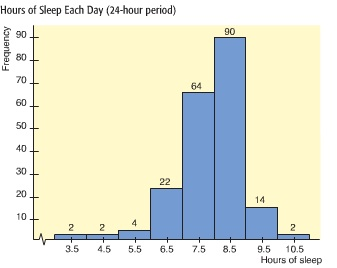
\includegraphics[scale=0.7]{WS4_HoursofSleep.jpg}
\end{center}

	\begin{enumerate}
	\item Estimate the mean number of hours of sleep. 

	{\answer{With $L_1 = \textnormal{ hours of sleep}$ and $L_2 = \textnormal{ frequencies}$, 
	1-Var Stats $L_1$, $L_2$ yields $\bar{x} = 7.9$ hours.}} 

	\item Estimate the standard deviation of hours of sleep. 
	(Is this a sample statistic or population parameter?) 
	
	{\answer{With $L_1 = \textnormal{ scores}$ and $L_2 = \textnormal{ frequencies}$, 
	1-Var Stats $L_1$, $L_2$ yields $s = 1.051440744$. 
	This is a sample statistic, since we have just a sample of subjects.}} 

	\end{enumerate}

\item The ogive shown represents the heights of males in a particular country in the 20-29 age group. \\

\begin{center}
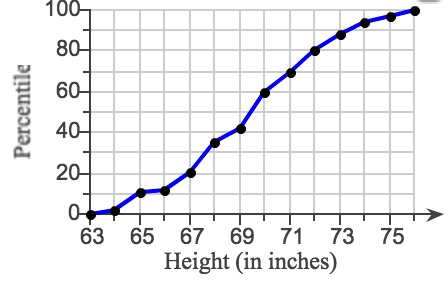
\includegraphics[scale=0.5]{WS5_Ogive.jpg}
\end{center}

	\begin{enumerate}
	%--
	\item Approximately what percentage of the males (age 20-29) are taller than 6 feet? 
	
	{\answer{The height of 6 feet (or 72 inches) looks to correspond to the 80th percentile. So, about 80\% of the males are 6 feet or shorter, leaving 20\% at a height of over 6 feet.}} 
	
	\item What is the approximate median height of this population of males? 
	
	{\answer{The median corresponds to the 50th percentile. According to the ogive, that falls somewhere between 69 and 70 inches}} 
	%--
	\end{enumerate}

\newpage

%Section 3.3 #11
\item {\em Consumer Reports} rated automobile insurance companies and listed annual premiums for top-rated companies in several states. The following figure shows box-and-whisker plots for annual premiums for urban customers (married couple with one 17-year-old son) in three states.

\begin{center}
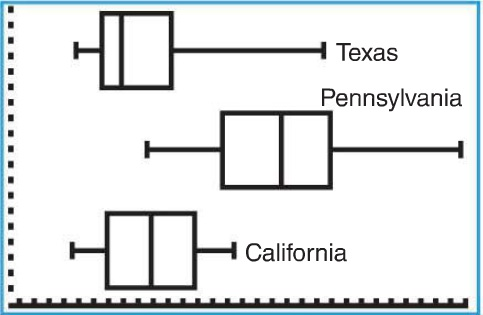
\includegraphics[scale=0.7]{WS5_InsuranceBox.jpg} 
\end{center}

	\begin{enumerate}
	\item Which state has the lowest annual premium? 
	
	{\answer{California - the low whisker, just slightly lower than Texas}} 
	
	\item Which state has the highest annual premium?
	
	{\answer{Pennsylvania - the high whisker}} 
	
	\item Which state has the highest median premium?
	
	{\answer{Pennsylvania - the line inside the box}} 
	
	\item Which state has the smallest range of premiums?
	
	{\answer{California - the smallest distance from low whisker to high whisker}} 
	
	\item Which state has the smallest inter-quartile range of premiums?
	
	{\answer{Texas - the smallest distance from lower box edges to upper box edge.}} 
	
	\end{enumerate}

\end{enumerate}	
\end{document}